%********************************************************************************
%       Preamble Information
%********************************************************************************
\documentclass[11pt, twocolumn]{article}
\usepackage[T1]{fontenc}
\usepackage[utf8]{inputenc}
\usepackage{mathpazo}
\usepackage{multicol}
\setlength\columnsep{20pt}

\usepackage{hyperref}
\hypersetup{
    colorlinks=true,
    linkcolor=blue,
    filecolor=magenta,      
    urlcolor=blue,
    citecolor=black
    }
% Used to include graphic images into LaTeX
\usepackage{graphicx}
% Tells the compiler to search in the images/ 
% folder for any included figures
\graphicspath{ {./images/} }

% Make lists more compact
% (from pandoc template)
\providecommand{\tightlist}{\setlength{\itemsep}{0pt}\setlength{\parskip}{0pt}}

% Prevent overfull lines
\setlength{\emergencystretch}{1em}

% No indentation and space between paragraph
\setlength{\parindent}{0.0in}
%\setlength{\parskip}{0.04in}
% Have space between paragraph
\setlength{\parskip}{11pt}

% Margin support
\usepackage[margin=0.75in]{geometry}

% header and footer
\usepackage{fancyhdr}

\newcommand{\thelabnumber}{HW3}
\newcommand{\thetitle}{HW3: Computer History}
% Update this line with your name 
\newcommand{\theauthor}{author1 \\ Dylan DeVault}

% Write title and author
\title{{\large } \thetitle}
\author{\theauthor}
\date{\today}

\pagestyle{fancy}
\fancyhf{}
\fancyfoot[R]{\thepage}
\fancyfoot[C]{HW3}
\fancyfoot[L]{CSE/IT 101 HW3}
\renewcommand{\footrulewidth}{1pt}
\renewcommand{\headrulewidth}{0pt}
\fancypagestyle{firstpage}{%
  \fancyhf{}% clear default for header and footer
  \fancyfoot[R]{\thepage}
  \fancyfoot[C]{HW3}
  \fancyfoot[L]{CSE/IT 101}
  \renewcommand{\footrulewidth}{1pt}
    \renewcommand{\headrulewidth}{0pt}
}

%********************************************************************************
%      Begin Document
%********************************************************************************
\begin{document}
\maketitle

\thispagestyle{firstpage}

%********************************************************************************
%      Report Content
%********************************************************************************
\section{Introduction}
Describe what topic you chose and why you chose that topic. Provide a summary of
the topic, in a general sense. This section should describe any background 
information that the reader needs to know to understand your topic.

\section{Time Period}
Describe the time period in which your topic was invented or used here. Also include
context for why your topic was used. Any specific historical information should be 
included here.

\section{Computer Hardware}
Describe the type of hardware that was used for your chosen topic.

Here, Figure \ref{fig:gpu} has been included so you have some code to use and update.
\begin{figure}
    \centering
    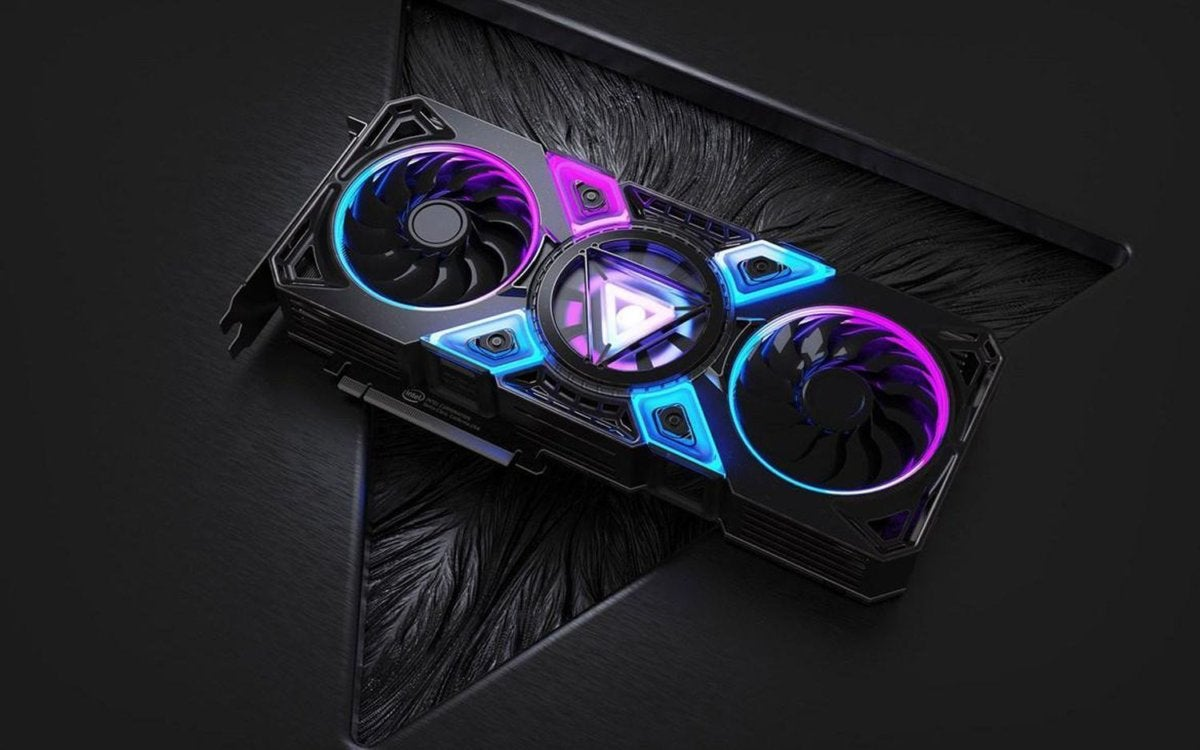
\includegraphics[width=0.45\textwidth]{gpu}
    \caption{Intel Arc GPU}
    \label{fig:gpu}
\end{figure}

I found this image on the PC World webpage \cite{Ung21}. 

\subsection{Computer Software}
The first tools to make AI was the programming language LISP also known as list processing. AI give the ability to think and preform tasks to robots. There is no commonly used software other than the modern programming languages and IDE's. There are multiple new ways of going about AI now like neural networks and generational development.

\subsection{Conclusion}
In conclusion AI and robotics are a new and developing part of computer history. 

%********************************************************************************
%      Report Content
%********************************************************************************
\bibliographystyle{acm}
\bibliography{sources}

\subsection{References}
Where we got the most of the information

ComputerHistory.org 
-https://www.computerhistory.org/revolution/artificial-intelligence-robotics/13/293


\end{document}